\pagestyle{fancy}
\pagenumbering{arabic}
\chapter{Introduction}
\label{chap:introduction}


%Structuur volgens Erwin
% INLEIDING (10-15 p)
% Onderzoeksgebied (1-2 p)
% Motivatie, probleemstelling (3p)
% Overkoepelende doelstelling en 4 meer toegespitste onderzoeksvragen (0.5 p)
% Kort literatuuroverzicht over de belangrijkste thema's die in meerdere hoofdstukken terugkomen (fragiliteit, geweld, behavioral economics, risico, ...) (3p)
% Belangrijkste resultaten per paper en "contributie aan literatuur" (1-2 p)
% Belangrijkste methoden en waarom juist deze? (2p)
% Roadmap to the thesis (1 p)

\section{Problem Statement and Research Area}
% Onderzoeksgebied (1-2 p)
% Motivatie, probleemstelling (3p)

%https://nsdsguidelines.paris21.org/node/291
%https://papers.ssrn.com/sol3/papers.cfm?abstract_id=2622220


%markets:
%https://link.springer.com/article/10.1007/s10551-010-0402-8
%https://www.oecd-ilibrary.org/content/paper/5k49dfg9fb6d-en
%https://www.worldbank.org/en/topic/fragilityconflictviolence/overview

%problem statement/Hook
Over the past decades, the world has made tremendous progress in fighting poverty, but this progress has not happened everywhere in equal measure. Between 1990 and 2017 \todo{MV: updaten naar 2022?}, the share of people wordwide living under the absolute poverty line of \$1.90 a day fell from 36.2\% to 9.3\%, while the share of Africans below the poverty line decreased less dramatically: from 58.4\% to 40.4\% \citep{WorldBank2021}. Furthermore, because of population increase on the continent, the absolute number of Africans living in poverty has actually increased over this time, as has the proportion of the world's poor who live in Africa. Within Africa, poverty rates have not declined uniformly across countries, with some countries faring worse than others. This means that the global poor are increasingly concentrated in a limited number of countries. The World Bank expects that by 2030, up to two thirds of the world's extremely poor live in Fragile Conflict-affected settings, and mostly in rural areas \citep{WorldBank2019}. %This does not make this a localized issue: instability in one country may have effects throughout the region through increased numbers of refugees and proliferation of armed groups. Such flows may even destabilize countries further away. %Climate change is expected to increase this instability further \citep{Burke2009}.

This concentratation of the world's poor in settings that defy the global trend of sharply decreasing povery rates has implications for the way in which we think about development. First, it means that the focus should be at a local level to investigate the local dynamics that underlie (or are caused by) the lack of development. It also implies that a healthy dose of intellectual modesty is in order.\todo{is dit niet een beetje too much?} Achieving development may not be one question with one answer, but rather a puzzle with many pieces, some more important in some cases than in others. In this disseration I take such a local approach; I  present evidence gathered at the micro-level in three countries: Sierra Leone, Cameroon and the Democratic Republic of the Congo (DRC). Each of these areas face their different issues, so the focus of the work done in each of the countries is different.

%Sweet mama salone
Sierra Leone is an often-used example of a conflict-related country. In 2010, the year when the Sierra Leonean data for this thesis was collected, the largest development challenge was recovering from the civil war that lasted from 1991 until 2002. During the course of the conflict, it is estimated that over 50,000 people lost their lives, and even more were victimized by the widespread human rights violation, from mass rape to mutiliations, perpetrated by all sides of the conflict \citep{HumanRightsWatch1999a}. Youth played an important role in the conflict, both in the grievances that caused the conflict \citep[see e.g.][]{Peters1998,Richards2005,Peters2011}, as well as in the actual fighting during the conflict \citep{Humphreys2013}. After the war, youths in the country were still left with little chance due the economic fall out of the conflict.  Agriculture, the largest sector in the country was hard-hit, leading to a high depedence on imported foodstuffs \citep{FAO2005}. 

Chapter \ref{chap:slfootball} draws on a study done with youths who participated in a football tournament in Kenema, Eastern Sierra Leone. The study focuses on the impact that their experiences during the conflict have had on their behaviour, and discusses potential implications of this for their future economic success. 

%DRC
Where Sierra Leone can be labelled post-conflict, such labelling is more complicated in the case of the DRC. While the Second Congo was ended by a peace agreement in 2003, there are still armed groups active in the country. After years of conflict, daily life for many in the DRC is miserable. The country lags behind in terms of human development, ranking 175 on the Human Development Index \citep{UNDP2020a}. The enduring conflicts have also depressed agricultural production, by limiting rural households' access to financial assets, land and markets; worsening instutional quality; decreased state capacity and migration  \citep{Lecoutere2005, Vlassenroot}. In 2020, it was estimated that over 20 million people were facing acute food insecurity in the country \citep{FAO2020}. Life for women in the DRC is particularly bad, facing high rates of sexual and gender-based violonce (SGBV), particularly from intimate partners; \cite{Peterman2011} estimate that 22.8\% of Congolese women have been victim of Intimate Partner Violence (IPV), and speculate that that may be an underestimate.

%\todo{MV:wat uit balans zo met de beschrijving van de SL studie, wellicht iets meer woorden aan geven, waar gaat het hfst op in, wat vind je?}
Chapters \ref{chap:n2a_impact} and \ref{chap:congogbv} draw on work done in South Kivu, one of the poorest provinces of the DRC \citep{Ansoms2009}. Chapter \ref{chap:n2a_impact} evaluates the outcomes of a project aimed at increasing agricultural production through the provision of input subsidies. The chapter presents evidence that the input subsidies succeeded in increasing adoption of inputs, but no evidence of effects on yields or food security is found. Chapter \ref{chap:congogbv} focuses on the drivers of SGBV. The chapter explores the characteristics of women who have been recently victimized by SGBV; I find that these women are less likely to have a high status within their household, and are less likely to have attended secondary education. I argue that this goes against notions that in order to stop SGBV in DRC bringing an end to the violence would be enough; rather, the incidence of SGBV is linked to the inferior position women have in the DRC, and this needs to be addressed in order to bring down incidence rates of SGBV.

%adamawa
%\todo{Expand the bit on Adamawa}
%\todo{MV: ook deze is wat uit balans. dit slaat volgens mij op hfst 4, zou ik noemen om consistent te blijven en ook wat uitwijden, zodat het meer in balans is}
Chapter \ref{chap:cameroontrust} is set in the Adamawa region in Northern Cameroon. The Adamawa region is mostly rural, with low population densities. The predominant source of income is agriculture. The most important challenge to development for the region is its remoteness. Most households in our study sample live in small villages, which means that they lack access to markets and the opportunities to development they entail. The chapter is based on the results of an Investment Game, a behavioural game commonly used to measure expectations about other people's behaviour, an important component of trust and thus of social capital. The paper focuses on the differences in determinants of behaviour in the game between respondents in village with markets access and those in villages without.




\todo{add paragraph conclusion?}

\section{Research Question}
% Overkoepelende doelstelling en 4 meer toegespitste onderzoeksvragen (0.5 p)
\todo{Write this into a story}
While the three research areas face different challenges, there is a common thread in their experiences with development. Each area faces certain risks and opportunities, and in each area different development outcomes are seen as priorities. The effect of each of these risks and opportunities on development outcomes is not direct. The effect is mediated through factors at the local or even the individual level, which in Figure \ref{intro:fig:framework} I capture under the term Social Capital and Institutions (for a more thorough review see below). \todo{MV: misschien goed om in section 1.1 al wat van deze termen te laten vallen, dan wordt er al een mooi bruggetje opgezet naar het theoretische deel in sectie 1.3} The chapters of this dissertation each discuss a different aspect of the interplay between risks, opportunities, social capital and development outcomes. The questions they answer are as follows.
\begin{enumerate}
	\item What is the relationship between conflict and competitive behaviour? (Chapter \ref{chap:slfootball});
	\item What is the effect of input subsidies on novel technology adoption? (Chapter \ref{chap:n2a_impact}
\ref{chap:cameroontrust});
	\item What is the effect of market access on trusting behaviour (Chapter \ref{chap:n2a_impact}
\ref{chap:cameroontrust}); and,
	\item What are the drivers of sexual and gender-based violence in Eastern Congo (Chapter \ref{chap:congogbv}).
\end{enumerate}


\section{Literature Review}
% Kort literatuuroverzicht over de belangrijkste thema's die in meerdere hoofdstukken terugkomen (fragiliteit, geweld, behavioral economics, risico, ...) (3p)
Figure \ref{intro:fig:framework} outlines the relationships between the main topics of this dissertation. On the right-hand side, there are two indicators for development that are present in the areas of interest in this disseration: human rights and (agricultural) productivity. On the left, there are three risks and opportunities: violent conflict, markets, and development aid. These risks and opportunities do not translate directly in development outcomes; rather, they are mediated through social capital and institutions.

\begin{figure}[htb]
  \centering
  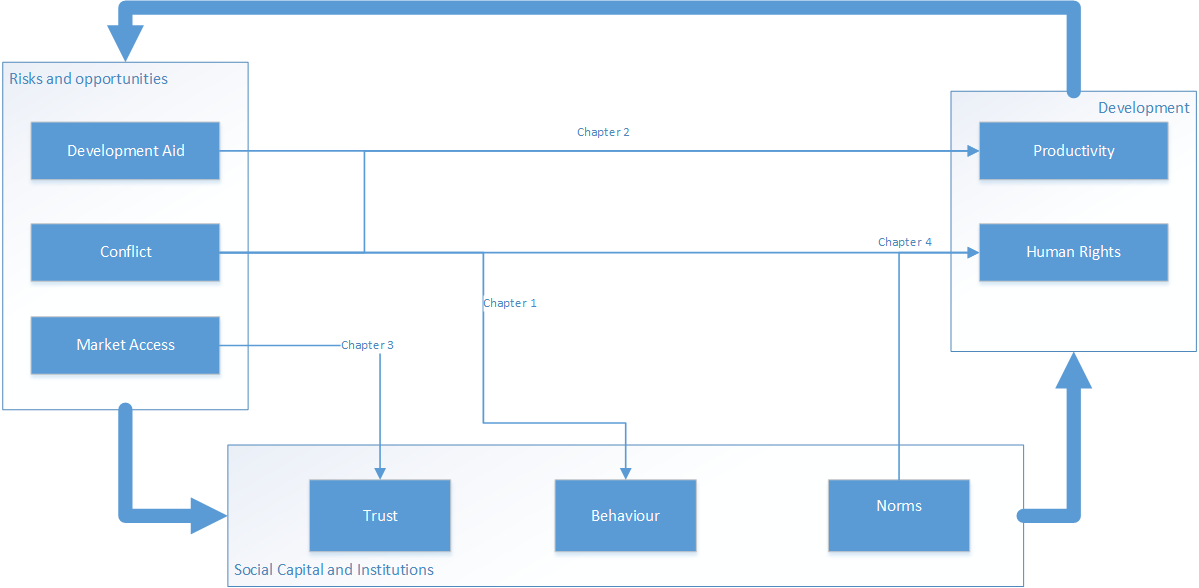
\includegraphics[width=0.8\linewidth]{"\git/thesis/analysis/introduction/figures/conceptual_framework.png"}
  \caption{Conceptual Framework}
  \label{intro:fig:framework}
\end{figure}

\subsection{Risks and Opportunities}
The first risk to development I consider is violent conflict. \citet{Collier2003}  expresses the risk posed by conflict to development by labelling it ``Development in Reverse''. The World Bank further underscored the importance of violent conflict in shaping development outcomes by titling their 2011 World Development Report ``Conflict, Security, and Development'' \citep{WorldBank2011}. Aside from the human rights violations that are inherent to violent conflict, other consequences include: decreased economic activity \citep{Collier1999} deforestation \cite[e.g.][]{Connectiona}, long-term incidence of domestic violence \citep[e.g.][]{LaMattina2017, Muller2019}, (mental) health problems \cite[e.g.][]{Smith2002, Iqbal2006a,Akresh2011} and food insecurity \cite[e.g.][]{Lecoutere2005, Verwimp2012}. However, some effects which may have some benefit to long-term development have been described, such as increased collective action \citep{Bellows2009b}, political participation \citep{Blattman2009a} and increased pro-social behaviour \citep{Voors2012a}.

Among the countries where data collection was done for this dissertation, two have a recent history of conflict: Sierra Leone and DRC. The conflicts have had far-reaching effects. In Chapter \ref{chap:slfootball}, I examine some of the impacts that conflict has had on the behaviour of youths in Sierra Leone, in particular with respect to their willingness to engage in competitive behaviour. Such competitiveness is crucial in shaping economic outcomes and productivity, and a such plays an important role in development \citep{Niederle2007}. Childhood and adolescence are a crucial time in the development of such preferences \citep{Benenson2007,Fehr2008,Sutter2007a}, and intense shocks such as conflict that happen during this time may thus have a large impact. We test this using a set of behavioural games in a population of Sierra Leonean youth.

%CongoGBV
The conflict that has persisted in the DRC for the past decades is often seen as the root cause for the high rates of SGBV that are the focus of Chapter \ref{chap:congogbv} \citep{Baaz2013,Kirby2015,Johnson2010}. However, \cite{Peterman2011} find that most SGBV is perpetrated by intimate partners, which casts doubts on the role of conflict as the main driver of the problem. In Chapter \ref{chap:congogbv} I draw on detailed survey data to find the background characteristics of victims of SGBV, allowing me to draw conclusions about the potential drivers of SGBV in Eastern DRC.

Next, I consider an opportunity for development: markets. Markets provide opportunities for exchange and specialization, which can boost economic development. At the national level, trade is seen as a promising way to increase productivity in developing economies. Dutch development aid, for example, has a large focus on the complementarities between trade and development as a way of increasing investments and thus productivity \citep[see e.g.][]{Zoomers2014}. Aside from these impacts on the national level, increased access to markets have been shown to have effects at the local and individual level as well: markets are associated with trust \citep{Tu2010,Fischer2008}; increased rationality \citep{List2008,Cecchi2013,Braga2009} and decreases in risk aversion \citep{Melesse2015}. This corresponds with findings that from large-scale societies (which include markets) engage more in pro-social behaviour \cite{Henrich2005,Henrich2010}. These national and individual effects make that markets are an important consideration in analysing the development process. 

This association of markets with increased rationality and increased pro-social behaviour should have effects on the behaviour in an investment game, which is determined to a large extent by expectations and pro-social preferences \citep{Berg1995,Ashraf2006,Roth1995,Sapienza2013}. In Chapter \ref{chap:cameroontrust} we test this by implementing an investment game as part of large-scale survy in Northern Cameroon, where some villages have good market access, while others are remote.


%put in for development aid vs institutional reform: https://www.aeaweb.org/articles/pdf/doi/10.1257/jel.44.4.973
Thirdly, I consider development aid. At the turn of the century, the Millennium Development Goals were adopted in the hopes that the world's poorest countries (particularly in Africa) could be lifted out of poverty with a large-scale international effort. The underlying assumption was that a core challenge to African economies were adverse geographical conditions which hinder growth; ambitious investments by the international development community could then help increase agricultural productivity and decrease the impact of tropical diseases \citep{Sachs2005}. This push came out of disappointment with the levels of growth in the 1990s. The mantra of "stabilize, privatize and liberalize", as preached by the IMF and the World Bank, proved insufficient to achieve preferred development outcomes, leading to calls  for an increase in the levels of development aid \citep{Rodrik2006a}. However, increased calls for more direct intervention were not the only response to this disappointment: concurrently there was doubt about development aid's capability to achieve meaningful growth. \citet{Easterly2007} claimed that Development Assistance was a ``mistake'', and that ``we don't know what actions achieve development'' \todo{MV: Pagina ref toevoegen}. A large literature has since sprung up that aims to fill exactly that knowledge gap and find out which development interventions work, and which don't. Improvements in statistical techniques and data collection methods have allowed development economists to get more accurate assessments of the impact of aid programs. Academics and development NGOs have embraced methods such as Randomized Controlled Trials (RCTs) to find out what works and what doesn't \citep[see e.g.][]{Bannerjee2011}.  

This dissertation follows in this tradition. Chapter \ref{chap:n2a_impact} is about the impact evaluation of an agricultural intervention, and both Chapters \ref{chap:cameroontrust} and \ref{chap:congogbv} were funded by being smaller parts of similar impact evaluations. This reflects the increased amount of field research that is being funded through evaluations of development aid, allowing economists to more accurately determine what actions work and which don't. 

\todo{dubbelcheck of dit niet theoretischer moet? Opzetje in comments}
%chapter 3: conflict has contribtued to low porductivity. 
%Sub-Sahara African countries show (very) low adoption rates of new agricultural technologies.
%Fertilizer use and improved seeds are strongly associated with increased levels of agricultural yields and productivity and providing such inputs at below market prices was long seen as a key element to propel farm households onto a sustained path of economic development and increased levels of food security

%chapter \ref{chap:n2a_impact} combines this with markets.

\subsection{Social Capital and Institutions}
The impact that these risks and opportunities can have differs across countries. Some countries have been better able to exploit the advantages markets offer than others; one conflict-affected country rebounds more quickly than another (compare for example the fortunes of Rwanda and the DRC). The key factor that sets apart countries that are successful in avoiding risk and capitalizing on opportunities is their institutional environment \citep{Rodrik2004,Acemoglu2000}. This term is used to describe the rules and norms that shape (economic) life. It covers crucial things such as protection of property rights and equal treatment by the law \citep{Acemoglu2005}. Such good institutions  foster development by incentivizing innovation. %However, the relationship between institutions and development does not run in one direction. While institutions cause growth \citep{Acemoglu2000}, the economic growth that accompanies development also allows for better institutions. It is possible that countries could enter a virtuous cycle, where improved institutional quality enhances growth, which improves institutional quality \citep{Voors2011}.

It is important to note that such institutions do not only include the formal rules and organizations which organize our lives; it includes informal arrangements shaped by the relations and networks between people as well. Insofar as these relations and networks provide value, they are termed social capital \citep[see for a more detailed discussion of the definition of the term][]{Putnam2001}. Especially in poorer countries, social capital plays an important role in facilitating economic activity, by providing a substitute for formal institutions \citep{Knack1997}. For example, kinship networks may provide insurance \citep{DiFalco2011}, while informal mechanisms may be more efficient at securing property rights than formal ones \citep{Platteau1996}. 

This insight, that social behaviours substitute for formal institutions in facilitating development, suggests that is not just international and national factors that drive development. Rather, relationships and behaviours at the local level may play an important role in shaping outcomes. This means that micro-level data collection is of importance for studying development. 

In this dissertation,  \todo{Schrijf dit uit.}

%fotball: studies the link between violent conflict and competitive behaviour. This behaviour is important...

%markets: ....

This dissertation contributes to this, by studying the links between behaviour and conflict (Chapter \ref{chap:slfootball}) and between behaviour and markets (Chapter \ref{chap:cameroontrust}).

%add in cardenas.

\subsection{Development}
As for development, I focus on agricultural productivity and human rights. This choice is ideosyncratic; it was driven by not by a grand notion of which issues matter most in the world, but it was driven by the NGOs who often cooperate on the projects underlying this dissertation. That is not to say these aren't important issues world wide. The focus on agricultural production is driven by the fact that the poorest of the world often depend on subsistence agriculture. Furthermore, agricultural productivity is seen as a necessary precondition for further, economy-wide, productivity improvements \citep{WorldBank2008}. However, few NGOs solely focus on productivity, as such a focus is too narrow to fully capture the problems associated with poverty. Productivity gains mean little in the face of widespread human rights violations. Human dignity is a crucial part of development. In addition to agricultural productivity, I focus on human rights as well; in particular women's rights. Two chapters from this dissertation deal with projects in the Congo, where many projects deal with women's rights. \todo{MV: prima als de exacte resultaten later komen in "findings" maar ik zou hier dan wel aangeven welke theorie je toetst in een behaald hoofdstuk}

\section{Findings}
% Belangrijkste resultaten per paper en "contributie aan literatuur" (1-2 p)
The key contribution of this thesis is the application of large-n data collection to questions on drivers of development in locations where such data collection is often difficult. The discussion on these drivers above revolves around many local dynamics, such as social capital, institutions and behaviour that are difficult to measure at higher aggregate levels. However, collecting data at lower levels, through household surveys, is often difficult and costly, precisely due to other dynamics considered here, such as lack of market access and conflict. By drawing on work done as part of increased efforts to measure the impact of development programs, this thesis presents local evidence from a variety of contexts, allowing a rich and detailed picture on development.

I find that the links between risks, opportunities and development are rarely straightforward. Conflict, for example, has effects on behaviour, which in turn may affect development in unforseen ways. In chapter \ref{chap:slfootball} I present \todo{MV: je wisselt tussen I en we, consistent maken?} evidence that conflicted-affected youth in Sierra Leone are more likely to receive a foul card during a football game, more less averse,  more altruistic towards their team-mates and more willing to compete towards members of competing football teams. These findings are in line with existing literature, and may have implications for post-conflict development. 

That is of course not to say that conflict is a positive thing for development. The scars of conflicts remain visible in both Sierra Leone and DRC today, even to the most casual observer. Even so, care should be given when attributing all problems that these countries face to the violent conflicts they underwent. One such problem is the high incidence of SGBV in Eastern DRC. Perpetration of SGBV by armed groups -- as a ``weapon of war'' -- is often seen as a crucial part of this high incidence. However, empirical evidence suggests that most SGBV is done at the hands of intimate partners \citep[see e.g.][]{Peterman2011}. Chapter \ref{chap:congogbv} complements this literature by examining the characteristics of female victims of SGBV. I find that victims are likely to be married to higher-status men and have low intra-household bargaining power. While the victims are more likely to have been exposed to violent conflict to the extent where they have lost family or household members before 2012 than non-victims, I find no link with more recent conflict history. This suggests that the issue of SGBV runs deeper than its framing as ``weapon of war'' suggests, and that  in order to address SGBV the position of women in Congolese society needs to be improved.

Chapters \ref{chap:n2a_impact} and \ref{chap:cameroontrust} look at opportunities to development: markets and development aid. With respect to development aid, in chapter \ref{chap:n2a_impact} I present evidence from an impact evaluation for a project subsidizing agricultural inputs in Eastern DRC. The evaluation found evidence that the project was successful in increasing input use among farmers: fertilizer use increased by five percentage points while use of inoculant (a novel technology aimed at increasing the amount nitrogen in the soil) increased by three percentage points. Considering the low rates of adoption in the region, these increases are large. However, we find no evidence of increased yields, or improved food security. Furthermore, we found that the improvements in input use took place in villages close to input market; in villages that were more remote uptake rates were unaffected by the subsidy program. This suggests an important role for market access in development.

That this role of market access goes beyond supplying goods vital to development is the finding of Chapter \ref{chap:cameroontrust}. We find that people living in communities with markets behave differently in an investment game. Specifically, in addition to social preferences, expectations of returns (a common indicator of trust) play a crucial in determining the amount they send. In non-market communities the amount sent is only determined by social preferences. 	Such trust facilitates a wide range of transactions and therefore plays an important role in development.

\section{Methods}
A common thread in all the chapters of this dissertation is the use of large-scale data collection combined with novel methods to collect data that would otherwise be hard to observe to observe. In particular, each chapter makes  use of experiments to measure aspects that are difficult to measure without bias using traditional methods. This includes concepts such as competitiveness and intra-village trust.

To measure the social preferences and competitiveness of the Sierra Leonean football players who are central in the research presented in Chapter \ref{chap:slfootball}, I use a range of behavioural games, most prominently a standard dictator games to measure other-regarding preferences and and effort game based on \citet{Niederle2007} to measure competitiveness.  

In Chapter \ref{chap:cameroontrust} I combine an Investment Game \citep{Berg1995} with a large scale survey to find the determinants of trusting behaviour. Such preferences would be impossible to measure without bias using survey questions, and given their importance in shaping social capital, the use of these experiments is vital in development economics \citep[see e.g]{Camerer1995, Cardenas2008a}.

The experiment of chapter \ref{chap:n2a_impact} is larger in scale. The works draws on an RCT, where rather than assigning individuals to experimental conditions, like in the behavioural games of the preceding chapters, entire villages are assigned to either a treatment condition (where they receive a subsidy) or a control condition (where they receive no such subsidy).

Finally, chapter \ref{chap:congogbv} relies on a list experiment to measure the incidence of Sexual and Gender-based Violence (SGBV)\todo{check abbreviations} while avoiding social desirability bias. This bias would be present in regular survey questions, because women are unlikely to talk to an interviewer about a sensitive topic like victimization. The list experiment removes this bias by removing the possibility of the interviewer (and researcher) to infer the victimization status of any individual respondent. This is done by presenting half the respondents with four problems and asking them how many of these problems they personally face. The other half of the women are presented with five problems: the same four, plus SGBV. An unbiased estimate of incidence of SGBV can thus be obtained by comparing the mean number of problems faced by both groups, as any such difference must be caused by SGBV incidence. 

The ability to get unbiased estimates of competitiveness, trust, program impact or SGBV incidence is of great importance where such localized \todo{MV: open einde}

\section{Roadmap}
% Roadmap to the thesis (1 p)
This dissertation is structured as follows. Following this introduction, there are four chapters, each presenting results from a different research project. Chapter \ref{chap:slfootball} uses data collected during a street football tournament in Sierra Leone, and examines the effect of conflict exposure on behaviour; Chapter \ref{chap:n2a_impact} presents the results from a randomized controlled trial to assess the impact of input subsidies on agricultural production in Eastern DRC; Chapter \ref{chap:cameroontrust} presents evidence from an investment game in Cameroon; and Chapter \ref{chap:congogbv} discusses the determinants of SGBV in Eastern DRC. Following these four chapters, there are concluding remarks, synthesizing the lessons learned from each of these chapters.



%bibliography, this is needed for bibtex
\clearpage 
\bibliographystyle{chicago}
%path to .bib file (e.g. automatically exported by mendeley) DO NOT include the file extension!
\bibliography{\bibtex/Thesis}